\documentclass[handout,x11names]{beamer}
\usepackage{etex,beamerfoils}
\usepackage{array,pifont,amsmath,latexsym,epsfig,amsfonts,yfonts}
\usepackage{amstext,amsopn,amsxtra,amsgen,amsbsy,amscd,amssymb,dcolumn,graphicx,setspace,pgfplots,booktabs,natbib}
\usepackage[normalem]{ulem}
\usepackage[all]{xy}
\beamertemplatetheoremsnumbered
\setbeamertemplate{caption}[numbered]
\usetheme{Copenhagen}
\definecolor{NewBlue}{RGB}{4, 114, 155}
\definecolor{magenta}{cmyk}{0,1,0,0}
\usecolortheme[named=NewBlue]{structure}
%\usecolortheme[named=SkyBlue4]{structure}

\newcommand{\D}{\displaystyle}
\newcommand{\E}{\begin{eqnarray*}}
\newcommand{\F}{\end{eqnarray*}}
\newcommand{\EE}{\begin{eqnarray}}
\newcommand{\FF}{\end{eqnarray}}
\newcommand{\IZ}{\begin{itemize}}
\newcommand{\ZI}{\end{itemize}}
\newcommand{\EN}{\begin{enumerate}}
\newcommand{\NE}{\end{enumerate}}
\newcommand{\itemc}{\item[$\circ$]}
\newcommand{\IZdash}{\begin{itemize} \renewcommand{\labelitemi}{-}}
\newcommand{\tn}{\textnormal}

% New commands to assist Beamer
\newcommand{\itemi}{\item<1->}
\newcommand{\itemii}{\item<2->}
\newcommand{\itemiii}{\item<3->}
\newcommand{\itemiv}{\item<4->}
\newcommand{\itemv}{\item<5->}
\newcommand{\itemvi}{\item<6->}
\newcommand{\itemvii}{\item<7->}
\newcommand{\itemviii}{\item<8->}
\newcommand{\itemix}{\item<9->}
\newcommand{\itemx}{\item<10->}

\newcommand{\itemci}{\item[$\circ$]<1->}
\newcommand{\itemcii}{\item[$\circ$]<2->}
\newcommand{\itemciii}{\item[$\circ$]<3->}
\newcommand{\itemciv}{\item[$\circ$]<4->}
\newcommand{\itemcv}{\item[$\circ$]<5->}
\newcommand{\itemcvi}{\item[$\circ$]<6->}
\newcommand{\itemcvii}{\item[$\circ$]<7->}
\newcommand{\itemcviii}{\item[$\circ$]<8->}
\newcommand{\itemcix}{\item[$\circ$]<9->}
\newcommand{\itemcx}{\item[$\circ$]<10->}


\newcommand{\fr}{\frame}
\newcommand{\ft}{\frametitle}
\newcommand{\ons}{\onslide}
\newcommand{\tc}{\textcolor}

\pgfplotsset{height =7cm,compat=1.7,width=7cm,
    standard/.style={
    	unit vector ratio*=1 1 1,
        axis x line=middle,
        axis y line=middle,
        enlarge x limits=0.15,
        enlarge y limits=0.15,
        every axis x label/.style={at={(current axis.right of origin)},anchor=north west},
        every axis y label/.style={at={(current axis.above origin)},anchor=north east}
    }
}
\newcommand{\drawge}{-- (rel axis cs:1,0) -- (rel axis cs:1,1) -- (rel axis cs:0,1) \closedcycle}
\newcommand{\drawle}{-- (rel axis cs:1,1) -- (rel axis cs:1,0) -- (rel axis cs:0,0) \closedcycle}

\usetikzlibrary{patterns}
\usetikzlibrary{arrows}
\usetikzlibrary{shapes}

\renewcommand{\bibsection}{}

% Watermark example: https://texblog.org/2012/02/17/watermarks-draft-review-approved-confidential/
\usepackage{draftwatermark}
\SetWatermarkText{This content is protected and may not be shared uploaded or distributed.}
\SetWatermarkScale{0.25}
\SetWatermarkAngle{0}
\SetWatermarkColor[gray]{1.0}
\setbeamercolor{background canvas}{bg=}%transparent canvas

\title[RBC Modeling\hspace{2em}\insertframenumber/
\inserttotalframenumber]{Introduction to Real Business Cycle Modeling}
\author{Brian C.~Jenkins \\ ~ \\University of California, Irvine}

\begin{document}

\frame{\maketitle}

\fr{
\ft{Introduction}

\IZ
\item Recall the Solow growth model with stochastic TFP:
	\EE
	Y_t & = & A_t K_t^{\alpha}\label{eqn:production}\\ 
	C_t & = & (1-s)Y_t\\
	Y_t & = & C_t + I_t\\
	K_{t+1} & = & I_t + (1-\delta)K_t \label{eqn:capital}\\
	\log A_{t+1} & = & \rho \log A_t + \epsilon_{t+1}, \label{eqn:tfp_process}
	\FF
where $\epsilon_{t+1} \sim\mathcal{N}\left(0,\sigma^2\right)$.

\

\item The model generates business cycle-like fluctuations in output, consumption, and investment.

\ZI
}

\fr{
\ft{Introduction}

\IZ


\item Let's evaluate the performance of the model by doing the following:

\


	\EN
	\itemi Use actual TFP values for the US for $A_t$ in equation (\ref{eqn:production}) and simulate the other variables in the model.
	\itemii Compare simulated output, consumption, and investment data with the actual data
	\NE
	
\

\itemiii But keep in mind that the Solow model was not designed to explain business cycles.
\ZI

}

\fr{
\begin{figure}[h] \caption{\label{fig_013_intro_rbc_modeling_solow_gdp} \textbf{GDP.} The stochastic Solow growth model does a \emph{reasonably} good job matching GDP fluctuations for the US from April 1948 to April 2022. {\tiny Source: FRED}.}
\begin{center}\hspace*{-.5cm}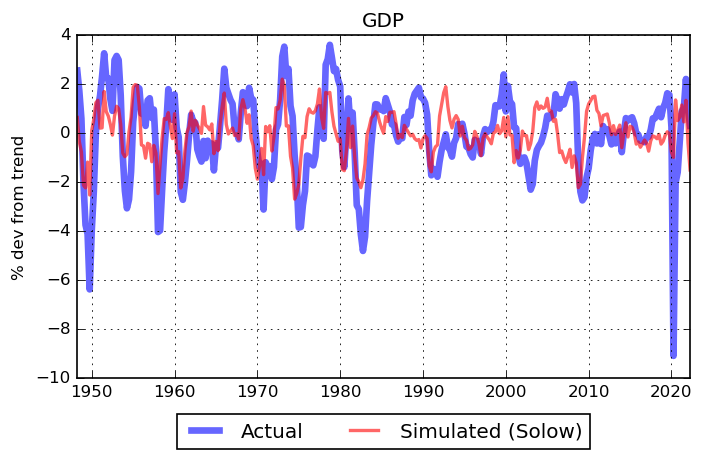
\includegraphics[height = 4.5cm]{fig_013_intro_rbc_modeling_solow_gdp.png}\end{center}
\end{figure}
}

\fr{
\begin{figure}[h] \caption{\label{fig_013_intro_rbc_modeling_solow_consumption} \textbf{Consumption.} The stochastic Solow growth model also does a \emph{reasonably} good job matching consumption fluctuations for the US from April 1948 to April 2022. {\tiny Source: FRED}.}
\begin{center}\hspace*{-.5cm}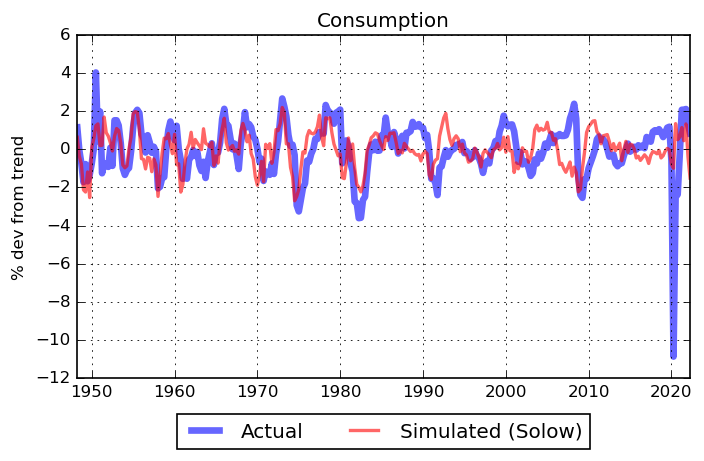
\includegraphics[height = 4.5cm]{fig_013_intro_rbc_modeling_solow_consumption.png}\end{center}
\end{figure}
}

\fr{
\begin{figure}[h] \caption{\label{fig_013_intro_rbc_modeling_solow_investment} \textbf{Investment.} The stochastic Solow growth model \emph{under-predicts} the magnitude of investment fluctuations for the US from April 1948 to April 2022. {\tiny Source: FRED}.}
\begin{center}\hspace*{-.5cm}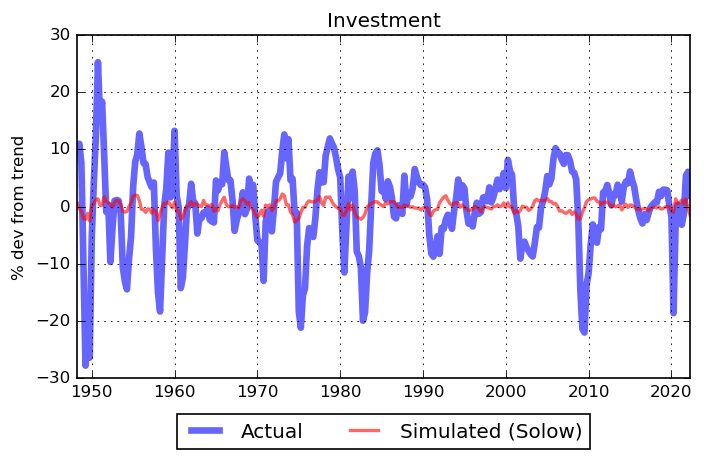
\includegraphics[height = 4.5cm]{fig_013_intro_rbc_modeling_solow_investment.png}\end{center}
\end{figure}
}





\fr{
\begin{table}[h] \caption{\label{tab013_intro_rbc_modeling_solow_stds} \textbf{Standard deviations.} Actual data and data simulated from stochastic Solow model. Units are percent deviations from trend. The model under-predicts the volatility of investment in particular. {\tiny Source: FRED}.}
\begin{center}\hspace*{-.5cm}

\begin{tabular}{lcc}
\toprule
{} &  Actual Data &  Simulated Data (Solow) \\
\midrule
Output      &         1.69 &                    0.93 \\
Consumption &         1.34 &                    0.93 \\
Investment  &         7.41 &                    0.93 \\
\bottomrule
\end{tabular}
\end{center}
\end{table}
}

\fr{
\begin{table}[h] \caption{\label{tab013_intro_rbc_modeling_solow_corrs} \textbf{Correlations with GDP.} Actual data and data simulated from stochastic Solow model. The model over-predicts the correlation of investment and consumption with GDP. {\tiny Source: FRED}.}
\begin{center}\hspace*{-.5cm}

\begin{tabular}{lcc}
\toprule
{} &  Actual Data &  Simulated Data (Solow) \\
\midrule
Consumption &         0.81 &                     1.0 \\
Investment  &         0.84 &                     1.0 \\
\bottomrule
\end{tabular}
\end{center}
\end{table}
}

\fr{
\ft{Introduction}

\IZ
\item Summary analysis of the stochastic Solow growth model:

	\IZ
	\itemii Simulated fluctuations of output and consumptionare comparable in scale to observed fluctuations
	\itemiii Under-predicts investment volatility
	\itemiv Over-predicts consumption-GDP and investment-GDP correlation
	\itemv No explanation for why labor fluctuates over the business cycle.	
	\ZI
	
	\
	
\itemvi \textbf{Objective}: Extend the model to improve performance.

\ZI
}


\fr{
\ft{Introduction}

\IZ
\itemi The model that \citet{Prescott1986} describes is an extension of the stochastic Solow growth model.

\

\itemii The most important differences are:

\EN
\itemii \textbf{Endogenous saving rate.} Consumption and investment decisions are made by a utility-maximizing \emph{representative household}.

\itemiii \textbf{Endogenous labor supply.} The utility-maximizing household chooses how much to work and therefore faces a labor-leisure tradeoff.
\NE

\

\itemiv Prescott's model is a \textbf{real business cycle} (\textbf{RBC}) model because it has no role for nominal quantities like inflation or nominal interest rates.

\ZI
}


\fr{
\ft{Introduction}

\IZ
\itemi We will ease into Prescott's RBC model in stages.

\

\EN
\itemii The \textbf{baseline} RBC model described in these slides:
	
	\IZ
	\itemiii \textbf{No labor supply choice}: household only chooses how much to consume and save.
	\itemiv \textbf{Centralized}: Household makes all production and allocation decisions. I.e., no firms, markets, or prices
	\ZI

\

\itemv In the next lecture, we'll add labor choice to the baseline model
\NE

\ZI
}


%\fr{
%\ft{Two-Period Model}
%
%\IZ
%\item A \emph{representative household} lives for a two periods.
%
%\
%
%\itemii The \emph{expected present value of lifetime utility} to the household from consuming $C_0$ and $C_1$ is $U_0$:
%	\EE
%	U_0 & = & \log (C_0) + \beta E_0 \log (C_1)\label{eqn:two_per_utility}
%	\FF
%	
%\
%
%\itemiii $0<\beta<1$ is the household's \emph{subjective discount factor}. (Annual model: $\beta \approx 0.96$. Quarterly model: $\beta \approx 0.99$)
%	
%\
%
%\itemiv $E_0$ denotes the \emph{expectation with respect to all information available as of date 0}.
%\ZI
%}
%
%
%\fr{
%\ft{Two-Period Model}
%
%\IZ
%\item The household enters period 0 with capital $K_0>0$.
%
%\
%
%\itemii Production in each period $t$:
%	\EE
%	F(A_t,K_t) & = & A_t K_t^{\alpha}
%	\FF
%where TFP $A_1$ is stochastic:
%	\EE
%	\log A_{1} & = & \rho \log A_0 + \epsilon_{1}
%	\FF
%	
%\
%
%\itemiii Capital depreciates at the constant rate $\delta$ per period.
%\ZI
%}
%
%\fr{
%\ft{Two-Period Model}
%
%\IZ
%\item The household faces the following sequence of budget constraints:
%    \EE
%    C_0 + K_1 & = & A_0 K_0^{\alpha}  + (1-\delta)K_0 \\
%    \pause C_1 & = & A_1 K_1^{\alpha}  + (1-\delta)K_1,
%    \FF
%where the boundary condition $K_2=0$ has been imposed.
%
%\
%
%
%\itemiii Note that in period 1, the household consumes both the output from the production function \emph{and} the undepreciated capital stock.
%
%\ZI
%
%}
%
%\fr{
%\ft{Two-Period Model}
%
%\IZ
%\item \textbf{Optimization problem}: In period 0, the household chooses:
%
%	\EN
%	\item Consumption for the current period
%	\item Capital for the subsequent period
%	\NE
%
%to maximize its expected present value of lifetime utility. 
%
%\
%
%\ZI
%}
%
%
%
%\fr{
%\ft{Two-Period Model}
%
%\IZ
%\item The household solves:
%	\EE
%	&&\max_{C_0,K_1} \; \log (C_0) + \beta E_0\log (C_1) \\\nonumber\\
%	&& \; \; \; \;  \; \; \; \; \tn{s.t.} \; \; \; \; C_0 + K_{1} \, = \, A_0 K_{0}^{\alpha}  + (1-\delta)K_0\nonumber\\
%	&& \; \; \; \;  \; \; \; \; \; \;\; \;\; \; \; \; \; \; \; \; \; \; \; \; \; C_1 \, = \, A_1 K_{1}^{\alpha}  + (1-\delta)K_1\nonumber
%	\FF 
%
%\
%	
%\itemii The problem can be written as a choice of $K_1$ only:
%	\EE
%	&&\max_{K_1} \; \log (A_0 K_{0}^{\alpha}  + (1-\delta)K_0 - K_1) \nonumber \\
%	&& \; \; \; \; \; \; \; \; \; \;   +\,  \beta E_0\log (A_1 K_{1}^{\alpha}  + (1-\delta)K_1)
%	\FF 
%
%\ZI
%
%}
%
%
%\fr{
%\ft{Two-Period Model}
%
%\IZ
%\item The first-order condition for the optimal choice of $K_1$ is:
%\EE
%    && \frac{1}{
%        \onslide<2-> \underbrace{ \onslide<1->
%        A_0 K_{0}^{\alpha}  + (1-\delta)K_0 - K_{1}
%        \onslide<2-> }_{C_0} \onslide<1->
%        } \nonumber \\
%	&& \; \; \; \; \; \; = \, \beta E_0 \bigg[\frac{\alpha A_1 K_1^{\alpha - 1} + 1 - \delta}{
%	\onslide<2-> \underbrace{ \onslide<1->
%	A_{1} K_{1}^{\alpha}  + (1-\delta)K_{1} - K_{2}
%	\onslide<2-> }_{C_1} \onslide<1->
%	}\bigg]
%    \FF
%    
%\
%
%\itemiii Or, more concisely:
%	\EE
%	\frac{1}{C_0} & = & \beta E_0 \left[\frac{\alpha A_{1}K_1^{\alpha - 1} + 1 - \delta}{C_1}\right]
%	\FF
%\ZI
%
%}
%
%\fr{
%\ft{Two Period Model}
%
%\IZ
%\item So given $K_0>0$ and $A_0$, the equilibrium paths for consumption, capital, and TFP are described described by:
%	\EE
%	\onslide<2->{\frac{1}{C_t} & = & \beta E_t \left[\frac{\alpha A_{t+1}K_{t+1}^{\alpha - 1} + 1 - \delta}{C_{t+1}}\right]}\\
%	\onslide<3->{C_t + K_{t+1} & = & A_{t} K_t^{\alpha} + (1-\delta) K_t}\\
%	\onslide<4->{\log A_{t+1} & = & \rho \log A_t + \epsilon_{t+1}}
%	\FF
%
%
%\ZI
%}


\fr{
\ft{Centralized RBC Model without Labor}

\IZ
\item A \emph{representative household} lives for an infinite number of periods.

\

\item The \emph{expected present value of lifetime utility} to the household from consuming $C_0, C_1, C_2, \ldots $ is denoted by $U_0$:
	\EE
	\pause U_0 & = & \log (C_0) + \beta E_0 \log (C_1) + \beta^2 E_0 \log (C_2) + \cdots\\
	\pause & = & E_0\sum_{t = 0}^{\infty} \beta^t \log (C_t),  \label{eqn:infinite_per_det_utility}
	\FF
	
\

\item $0<\beta<1$ is the household's \emph{subjective discount factor}. (For a quarterly model: $\beta \approx 0.99$ makes usually sense)
	
\

\item $E_0$ denotes the \emph{expectation with respect to all information available as of date 0}.
\ZI



}

\fr{
\ft{Centralized RBC Model without Labor}

\IZ
\item The household enters period 0 with capital $K_0>0$.

\

\itemii Production in period $t$:
	\EE
	F(A_t,K_t) & = & A_t K_t^{\alpha}
	\FF
where TFP $A_t$ is stochastic:
	\EE
	\log A_{t+1} & = & \rho \log A_t + \epsilon_{t+1}
	\FF
	
\

\itemiii Capital depreciates at the constant rate $\delta$ per period.
\ZI
}

\fr{
\ft{Centralized RBC Model without Labor}

\IZ
\item The household faces the following sequence of budget constraints:
    \EE
    C_0 + K_1 & = & A_0 K_0^{\alpha}  + (1-\delta)K_0 \\
    \pause C_1 + K_2 & = & A_1 K_1^{\alpha}  + (1-\delta)K_1 \\
    \pause C_2 + K_3 & = & A_2 K_2^{\alpha}  + (1-\delta)K_2 \\
    %\vdots \; \; \; \; \; \; & \vdots & \; \; \; \; \; \; \; \; \; \; \; \; \; \;  \vdots 
    & \vdots & 
    \FF



\itemiv Express the constraints more concisely as 
    \EE
    C_t + K_{t+1} & = & A_t K_{t}^{\alpha}  + (1-\delta)K_t, \label{eqn:infinite_per_det_bc}
    \FF
 for $t = 0, 1, 2, 3,\ldots$

\ZI

}

\fr{
\ft{Centralized RBC Model without Labor}

\IZ
\item \textbf{Optimization problem}: Each period the household chooses:

	\EN
	\itemii Consumption for the current period
	\itemiii Capital for the subsequent period
	\NE

	\onslide<3->{to maximize its expected present value of lifetime utility.}

\

\itemiv We'll solve the problem for period 0 and then generalize the solution to apply to all periods $0, 1, 2, \ldots$

\ZI
}



\fr{
\ft{Centralized RBC Model without Labor}

\IZ
\item In period 0, the household solves:
	\EE
	&&\max_{C_0,K_1} \; E_0\sum_{t=0}^{\infty}\beta^t\log (C_t) \\\nonumber\\
	&& \; \; \; \;  \; \; \; \; \tn{s.t.} \; \; \; \; C_t + K_{t+1} = A_t K_{t}^{\alpha}  + (1-\delta)K_t\nonumber
	\FF 

\
	
\itemii The problem can be written as a choice of $K_1$ only:
	\EE
	&&\max_{K_1} \; E_0\sum_{t=0}^{\infty}\beta^t\log ( A_t K_{t}^{\alpha}  + (1-\delta)K_t - K_{t+1})
	\FF 

\ZI

}


\fr{
\ft{Centralized RBC Model without Labor}

\IZ
\item Note:
	\EE
	&& E_0\sum_{t=0}^{\infty}\beta^t\log ( A K_{t}^{\alpha}  + (1-\delta)K_t - K_{t+1})\nonumber\\
	&& \; \; \; \; \; \; = \, \log(A_0 K_{0}^{\alpha}  + (1-\delta)K_0 - K_{1}) \nonumber \\
	&& \; \; \; \; \; \; \; \; \; \; \; \; + \, \beta E_0\log(A_{1} K_{1}^{\alpha}  + (1-\delta)K_{1} - K_{2}) \nonumber\\
	&& \; \; \; \; \; \;\; \; \; \; \; \;\; \; \; \; \; \; + \, [\text{terms independent of $K_1$}]
	\FF 
	
\

\itemii So:
	\EE
	\frac{\partial}{\partial K_1} U_0 & = &  -\frac{1}{A_0 K_{0}^{\alpha}  + (1-\delta)K_0 - K_{1}} \nonumber\\
	&& \; \; \; \;  + \, \beta E_0 \left[\frac{\alpha A_1 K_1^{\alpha - 1} + 1 - \delta}{A_{1} K_{1}^{\alpha}  + (1-\delta)K_{1} - K_{2}}\right]
	\FF 

\ZI

}

\fr{
\ft{Centralized RBC Model without Labor}

\IZ
\item Therefore the first-order condition for the optimal choice of $K_1$ is:
\EE
    && \frac{1}{
        \onslide<2-> \underbrace{ \onslide<1->
        A_0 K_{0}^{\alpha}  + (1-\delta)K_0 - K_{1}
        \onslide<2-> }_{C_0} \onslide<1->
        } \nonumber \\
	&& \; \; \; \; \; \; = \, \beta E_0 \bigg[\frac{\alpha A_1 K_1^{\alpha - 1} + 1 - \delta}{
	\onslide<2-> \underbrace{ \onslide<1->
	A_{1} K_{1}^{\alpha}  + (1-\delta)K_{1} - K_{2}
	\onslide<2-> }_{C_1} \onslide<1->
	}\bigg]
    \FF
    
\

\itemiii Or more concisely:
	\EE
	\frac{1}{C_0} & = & \beta E_0 \left[\frac{\alpha A_{1}K_1^{\alpha - 1} + 1 - \delta}{C_1}\right]
	\FF
\ZI

}

\fr{
\ft{Centralized RBC Model without Labor}

\IZ

\item The household solves the same problem in periods $1, 2, 3, \ldots$

\

\item So given $K_0>0$ and $A_0$, the equilibrium paths for consumption, capital, and TFP are described described by:
	\EE
	\pause \frac{1}{C_t} & = & \beta E_t \left[\frac{\alpha A_{t+1}K_{t+1}^{\alpha - 1} + 1 - \delta}{C_{t+1}}\right]\\
	\pause C_t + K_{t+1} & = & A_{t} K_t^{\alpha} + (1-\delta) K_t\\
	\pause \log A_{t+1} & = & \rho \log A_t + \epsilon_{t+1}
	\FF


\ZI
}


\fr{
\ft{Centralized RBC Model without Labor}

\IZ

\item Computing numeric values for consumption and capital is not trivial. Recall the Euler equation:
	\EE
	\frac{1}{C_t} & = & \beta E_t \left[\frac{\alpha A_{t+1}K_{t+1}^{\alpha - 1} + 1 - \delta}{C_{t+1}}\right]
	\FF
	
\

\item Consumption at date $t$ depends on the \emph{expectation} of consumption at date $t+1$ which in turn depends on the expectation of consumption at date $t+2$ and so on.


\

\item Solving the problem requires numerical methods like those employed in the \texttt{linearsolve} Python package.

\ZI
}


\fr{
\input{figure_013_intro_rbc_modeling_rbc_without_labor_irs.tex}
}


\fr{
\begin{figure}[h] \caption{\label{fig_013_intro_rbc_modeling_rbc_without_labor_gdp} \textbf{GDP.} Like the stochastic Solow model, the baseline RBC model without labor does a \emph{reasonably} good job matching GDP fluctuations for the US. {\tiny Source: FRED}.}
\begin{center}\hspace*{-.5cm}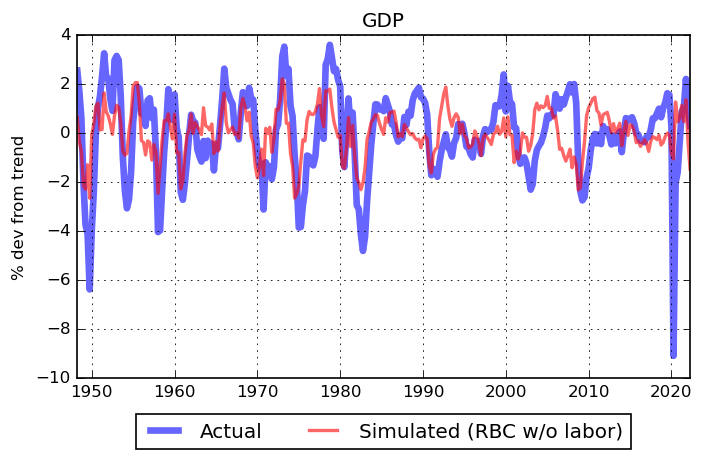
\includegraphics[height = 4.5cm]{fig_013_intro_rbc_modeling_rbc_without_labor_gdp.png}\end{center}
\end{figure}
}

\fr{
\begin{figure}[h] \caption{\label{fig_013_intro_rbc_modeling_rbc_without_labor_consumption} \textbf{Consumption.} In contrast to the stochastic Solow model, the baseline RBC model without labor \emph{under-predicts} the magnitude of consumption fluctuations for the US. {\tiny Source: FRED}.}
\begin{center}\hspace*{-.5cm}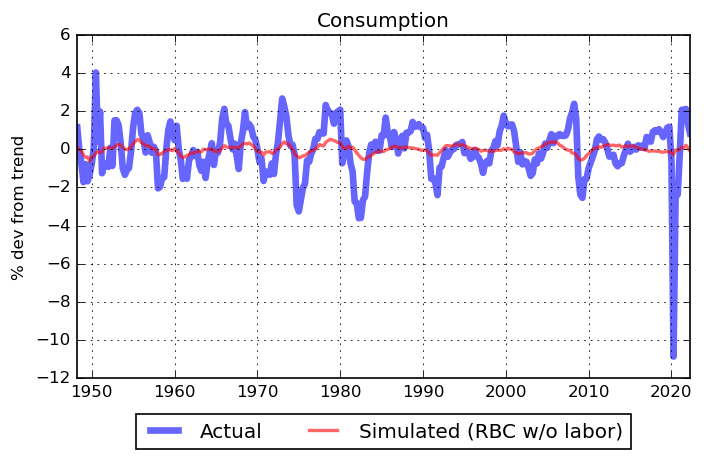
\includegraphics[height = 4.5cm]{fig_013_intro_rbc_modeling_rbc_without_labor_consumption.png}\end{center}
\end{figure}
}

\fr{
\begin{figure}[h] \caption{\label{fig_013_intro_rbc_modeling_rbc_without_labor_investment} \textbf{Investment.} The baseline RBC model does a \emph{reasonably} good job matching the magnitude of investment fluctuations better than the stochastic Solow model. {\tiny Source: FRED}.}
\begin{center}\hspace*{-.5cm}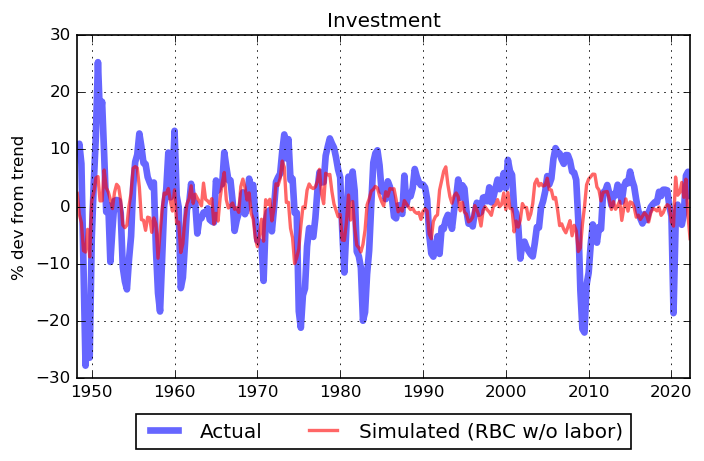
\includegraphics[height = 4.5cm]{fig_013_intro_rbc_modeling_rbc_without_labor_investment.png}\end{center}
\end{figure}
}


\fr{
\begin{table}[h] \caption{\label{tab013_intro_rbc_modeling_solow_rbc_without_labor_stds} \textbf{Standard deviations.} Actual data and simulated data. Units are percent deviations from trend. {\tiny Source: FRED}.}
\begin{center}\hspace*{-.5cm}

\begin{tabular}{lccc}
\toprule
{} &  Actual Data &  Solow &  RBC w/o Labor \\
\midrule
Output      &         1.69 &   0.93 &           0.94 \\
Consumption &         1.34 &   0.93 &           0.22 \\
Investment  &         7.41 &   0.93 &           3.39 \\
\bottomrule
\end{tabular}
\end{center}
\end{table}
}


\fr{
\begin{table}[h] \caption{\label{tab013_intro_rbc_modeling_solow_rbc_without_labor_corrs} \textbf{Correlations with GDP.} Actual data and simulated data. {\tiny Source: FRED}.}
\begin{center}\hspace*{-.5cm}

\begin{tabular}{lccc}
\toprule
{} &  Actual Data &  Solow &  RBC w/o Labor \\
\midrule
Consumption &         0.81 &    1.0 &           0.61 \\
Investment  &         0.84 &    1.0 &           0.99 \\
\bottomrule
\end{tabular}
\end{center}
\end{table}
}

\fr{
\ft{Centralized RBC Model without Labor}

\IZ
\item Summary analysis of the RBC Model without labor:

	\IZ
	\itemii Substantial improvement over the stochastic Solow model for explaining investment volatility
	\itemiii Substantially under-predicts consumption volatility (i.e., consumption is too smooth)
	\ZI
	
	\
	
\itemvi \textbf{Next}: Add a labor-leisure tradeoff to the household's problem.

\ZI
}

\fr{
\ft{References}
\bibliographystyle{aer}
\bibliography{comp_econ_references.bib}
}

\end{document}